\documentclass[]{article}
\usepackage{authblk}
\usepackage{caption}
\usepackage{microtype}
%\usepackage{amsthm}
\usepackage{graphicx}
\graphicspath{{figures/}}
\DeclareGraphicsExtensions{.pdf,.jpeg,.png}
%\usepackage{dsfont}
%\usepackage{amsmath}
%\usepackage{fancyvrb}
%\usepackage{color}
%\usepackage{algorithmic}
%\usepackage{array}
%\usepackage{mdwmath}
%\usepackage{mdwtab}
%\usepackage{eqparbox}
%\usepackage{fixltx2e}
%\usepackage{stfloats}
%\usepackage{float}
%\restylefloat{table}
%\restylefloat{graphicx}
\usepackage{url}
\usepackage{listings}
\usepackage{comment}

%opening
\title{}
\author{Yue Cai Zhu	}
%\authornote{Dr.~Trovato insisted his name be first.}
%\orcid{1234-5678-9012}
\affil{McGill University}
\affil {yue.c.zhu@mail.mcgill.ca}

\renewcommand\Affilfont{\itshape\small}

\begin{document}

\maketitle

\begin{abstract}

\end{abstract}

\section{Introduction}
Statistical Language Model(SLM) is a conditional probability distribution  of a sequence of linguistic  entities including words, phrases, characters.
It is widerly used to improve the performance of various natural language applications, such as speech recognition, text mining, spelling correction or recommendation and machine translation. 
The method to obtain a Statistical Language Model are well explored in the past 40 years\cite{rosenfeld1996maximum}\cite{breiman1984classification}\cite{jelinek1992basic}\cite{jelinek1992basic}.
Recently Mikolov et al. applied Recurrent Neural Network(RNN) in SLM and reported good performance\cite{mikolov2010recurrent}.
The model they applied is called the Elman network which is a simple kind of RNN and they believe that the ability of RNN to store past context is the key to its good performance.
However, the gradient vanishing problem\cite{hochreiter1998vanishing} in the training or the Elman network could potentially degrade its performance.  
The solution to this problem is a new type of RNN which is call Long Short Term Memory(LSTM)\cite{hochreiter1997long} and its variant Gated Recurrent Unit(GRU)\cite{cho2014properties}.
In this work, we are interested to see whether LSTM and GRU could outperform the Elman network in charactor level SLM, namely, is the gradient vanish problem is critical to charator level SLM.  


Moreover, previous work focus on word level SLM and not much progress has been made for charactor level SLM. 
It is well believed that charactor level SLM requires less train data than word level SLM but to the best of our knowledge no formal experiment to support this argument.
Therefore, we are also interested to varify this argument.

The contributions of this paper is listed below:
\begin{itemize}
	\item Compare the performance of LSTM and GRU to the Elman net and verify that the gradient vanishing problem is not critical in charactor level SLM. Moreover, because charator level SLM only need short term history, the Elman network is actually more suitable to charactor level SLM.
	\item Veriy that charactor level SLM requires less training data than word level SLM 
\end{itemize}

The organization of the paper is as the following: section 1 briefly introduce the motivation of this work; 
section 2 introduce the background of SLM and charactor level SLM and propsed the two research questions of this paper; 
section 3 introduce the detail of the three types of Recurrent Neural Network used in the experients which is the Elman network, LSTM and GRU;
section 4 describe the experiment design, the pen-tree bank data set used in the experiemnts and the perplexity that used to evaluate the performance of the resulted SLMs.
section 5 report the experiemtn result and answer the proposed research questions.
section 6 summarizes this work. 






\section{Background}


\subsection{Statistical Language Modeling}
In Natrual Language Processing(NLP), Statistical Language Model(SLM) is a probability distribution  of all possible sequence of linguistic  entities including words, phrases, characters\cite{rosenfeld2000two}. 
In Practice, a traditional task in SLM is to model the probability that a given linguistic  entity appears next after a given sequence of linguistic  entities. 
This could be defined as the conditional probability distribution $P(e_i| e_1,e_2,...,e_{i-1})$ of the next linguistic entities $e_i$ given a sequence of prior entities $(e_1,e_2,...,e_{i-1})$. 
%For example, given the sequence of words: "I love", an SLM may give out the possiblity of 70\% for the next word to be "you" and 5\% for the word "toilet". 

Statistical Lanuguage Model is generally used to improve the performance of speech recognition, text mining, spelling correction or recommendation and machine translation. 
For example, in automatic speech recognition, given an acoustic signal, the goal is to find the sentence that is most likely to have been spoken. 
In this process, SLM serves as a prior distribution in the classifier.
Figure \ref{speech_recognition} illustrates how SLM is applied in speech recognition.

\begin{figure}
	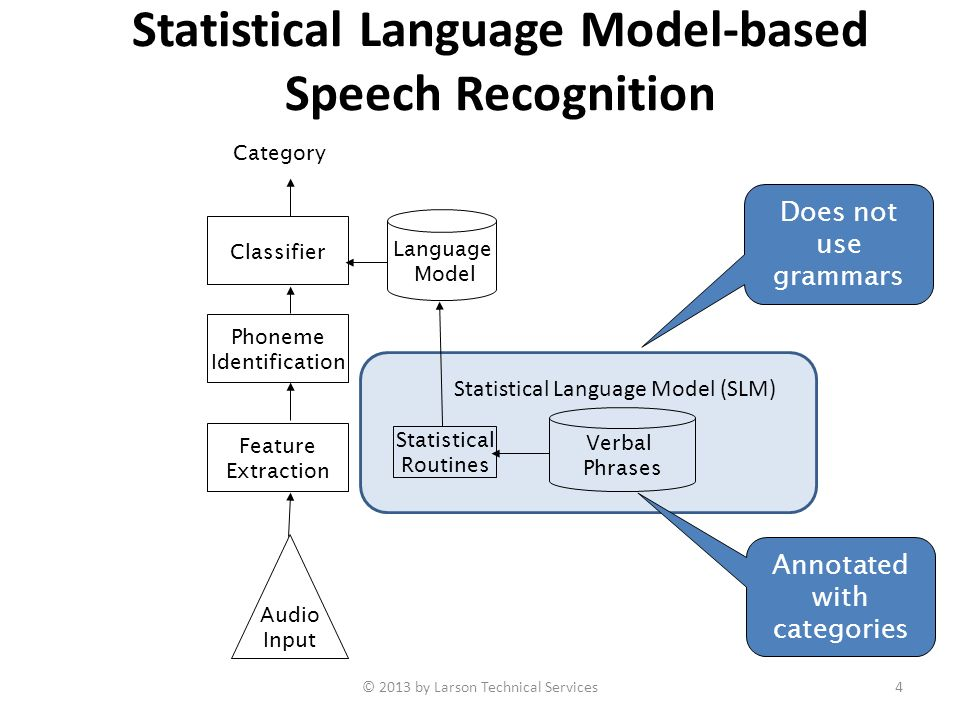
\includegraphics[scale=0.5]{speech.jpg}
	\caption{Speech recognition\cite{daniela2013speech}}
	\label{speech_recognition}
\end{figure}

\subsection{Charactor Level Language Modeling }
By Charactor level language model, we obtain the conditional probability distribution $P(c_i|c_1,c_2,...,c_{i-1})$ where $c_i$ is the charactor locates in the ith position of a charactor sequence. 
It captures the instrinsic rules of constructing a valid word by charactors.
Charactor level language model can be used together with word level language model to better handle poems and songs, it can also be used in spelling correction or recommendation.
It is believed that charactor level language model require less training data than word level model because the small vocabulary size.
However, this has not been formally verified.
Most of the previous work focus on word level modeling or phrase level.
Because they can make use the semantic information learned from documents to give out predictions which make sense to human. 
Not much work for charactor level language modeling except for some charactor based languages such as Chinese and Korean.




\subsection{Research Questions}
In this work, we are trying to answer the following two research questions.


\textbf{RQ1: Is Charactor Level Language Model Requires Less Training Data Than Word level?} 
One critical requriement of word level language modeling is the need of enormous amount of documents to train a good model to learned the syntactic rule of a particular language and the semantic information from a given document.
Moreover, some rarely used words would be ignored by the model because its small frequency in the documents.
We can only include more documents with the hope that the rarely used words could get enough frequency count to be captured.
In contrast, charactor level language model just need to learn the instrinsic rules of constructing a valid words, given the small size of the set of available charactors in a language, it should require much less documents to train a good model. 
But is this argument really true?
We can only verify this by experiments. 

\textbf{RQ2: Which Recurrent Network Is Better for Charactor Level Language Modeling?} 
Recurrent neural network is good in handling sequential data. 
Sentence and word are one type of sequential data. 
As shown by Mikolov et al.\cite{mikolov2010recurrent}, the Elman network could achieve exellent performance in language modeling.
But due to the gradient vanishing problem in training\cite{hochreiter1998vanishing}, the Elman network is less capable to remember long term history than Long Short Term Memory and Gated Recurrent Unit.
From the proposed argument in RQ1, charactor level language only need to learn the intrinsic rule of constructing words.
Is long term memory important for learning this intrinsic rule? 
Namely which Recurrent Network Is Better for Charactor Level Language Modeling?


\section{Methodology}
For the experiments, we implement the following three types of recurrent neural network: the Elman network, long short term memory and gated recurrent unit.


\subsection{The Elman Network}
The Elman network is one of the simplest recurrent neural network\cite{elman1990finding}. 
Its structure is shown in figure \ref{elman}.
\begin{figure}
	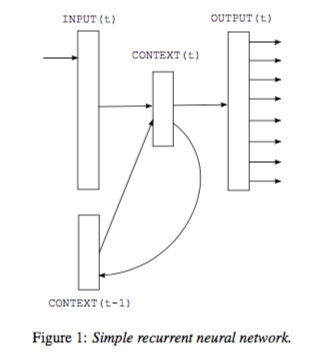
\includegraphics[scale=0.8]{elman.png}
	\caption{The Elman Network\cite{mikolov2010recurrent}}
	\label{elman}
\end{figure}

By adding the hidden context layer, the elman network is capable to take previous input together with the current input to give out prediction. 
Given the input embedding $w(t)$ at time $t$ of size $V$, the output layer concatenates the previous output of hidden context layer $s(t-1)$ of size $H$ as equation 1 to generate the output vector $x(t)$  of size $V+H$.
\begin{equation}
	x(t) = w(t)||s(t-1)
\end{equation}

where $||$ is the operation of concatenation. 
Then the output of the hidden context layer is updated by:
\begin{equation}
	s(t) = f(x(t)  \cdot u)
\end{equation}

where u is the weight for the hidden context layer and has size of $(V+H) \times H$ and $f()$ is the sigmoid function.
And $s(t)$ is also called the encoding of the recurrent network at time $t$ which will be passed to the output layer to generate the output $y(t)$:

\begin{equation}
	y(t) = g(s(t) \cdot v)
\end{equation}

where $v$ is the weight matrix for the output layer and has size of $H \times K$ given $K$ to be the size of $y(t)$. 
And $g()$ is the softmax activation function.
Notice that bias could be added to the updating of $s(t)$ and $y(t)$ in practice for more freedom in performance tuning.


The Elman network is capable to remember input history. 
However, due the the gradien vanishing/exploding problem, the impact of past history could eventually has no effect or takes major effect\cite{hochreiter1998vanishing}.
In order to solve this problem, another type of recurrent neural network which named long short term memory is proposed\cite{hochreiter1997long}.



\subsection{LSTM}
Long short term memory adds the input gate $i_t$, forget gate $f_t$ and output gate $o_t$ to control the remaining of backpropagated error which continuously feeds error back to each of the three gates until they learn to cut off the value. 
Thus, regular backpropagation is effective at training an LSTM unit to remember values for long durations.
Its structure is shown in figure \ref{lstm}.

\begin{figure}
	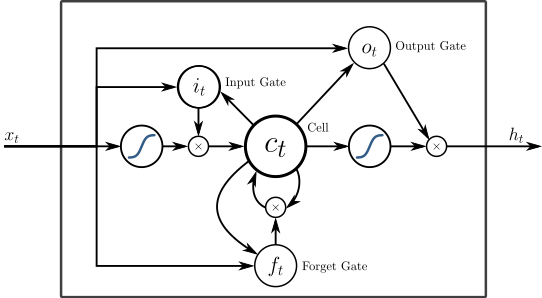
\includegraphics[scale=0.65]{lstm.png}
	\caption{Long Short Term Memory\cite{hochreiter1997long}}
	\label{lstm}
\end{figure}
Given the input vector $x_t$ at time $t$, the output gate $f_t$ is updated as:
\begin{equation}
	f_t = \sigma_g(W_fx_t + U_fh_{t-1} + b_f)
\end{equation}

The input gate $i_t$ is updated as:
\begin{equation}
	i_t = \sigma_g(W_ix_t + U_ih_{t-1} + b_i)
\end{equation}

And the output gate $o_t$:
\begin{equation}
o_t = \sigma_g(W_ox_t + U_oh_{t-1} + b_o)
\end{equation}

then the context layer $c_t$ is updated as:

\begin{equation}
c_t = f_t \circ c_{t-1} +i_t \circ \sigma_c(W_cx_t + U_ch_{t-1} + b_c)
\end{equation}

after the hidden context layer is updated, the output of the network is obtained by:
\begin{equation}
	h_t = o_t \circ \sigma_h(c_t)
\end{equation}

where $W$ , $U$ are the weight matrix for the corresponding gate,  $\circ$ is the point wise product operation and $\sigma$ is the sigmoid function .


\subsection{Gated Recurrent Unit}

GRU is proposed to solve the gradient vanishing problem in training a (RNN)\cite{chung2014empirical}.
It acheive the same performance as Long Short Term Memory but with less computations.
Its stucture is show in figure \ref{gru}. $h$ is the current state and $\hat{h}$ is context state which could memorize the impact of the input history. 
The reset gate $r$ controls whether the state from the current input should be memorized in $\hat{h}$.
The update gate $z$ controls whether the memory from $\hat{h}$ should considered when updating $h$ to give out prediction.  
\begin{figure}
	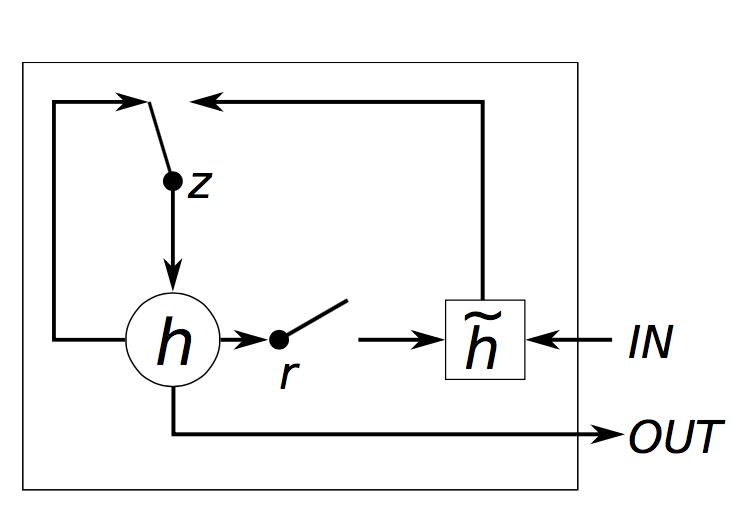
\includegraphics[scale=0.8]{gru.png}
	\caption{Gated Recurrent Unit\cite{chung2014empirical}}
	\label{gru}
\end{figure}

Given the input vector $x_t$ at step t, each gates and states are calcuated recursively as:
\begin{equation}
z_t = \sigma_g(W_zx_t+U_{z}h_{t-1}+b_z)
\end{equation}	
\begin{equation}
r_t =  \sigma_g(W_rx_t+U_{r}h_{t-1}+b_r)
\end{equation}	
\begin{equation}
h_t=(1-z_t) \circ h_{t-1} + z_t \circ \sigma_h(W_hx_t+U_{h}(r_t \circ h_{t-1})+b_h)
\end{equation}
Where $o$ is point-wise multiplication, $W$ and $U$ is the weight matrices for the corresponding component, $b$ is the bias vector.
$\sigma_g$ is the sigmoid activation function which has the form:
\begin{equation}
\sigma_g(x) = \frac{1}{1+e^{-1}}
\end{equation}
and $\sigma_h$ is the hyperbolic tangent activation function with the form:
\begin{equation}
\sigma_h(x)=\frac{e^x - e^{-x}}{e^x + e^{-x}}	
\end{equation}

\section{Experiment Design and Evaluation}


\subsection{Data and Settings}
We use the Penn TreeBank data set in our experiment. 
The Penn TreeBank data set is commonly used to evaluate statistical language models.
It is generated from 2,499 Wall Stree stories which have in total $1,000,000$ words and a vocabulary of size $10,000$.
There are $49199$ sentences in the data set and they are separed to three data set, the training, validating and testing data set.
The training data set has $42068$ sentences with $887521$ words.
The validating set has $3370$ sentences with $70390$ words. 
And the testing set has $3761$ sentences with $78669$ words.


All neural network are train with the same settings with the same structure which consists of two hidden states of size $1500$.
They are trained in 10 epochs with batch size of 80. 
The initial learning rate is 1 and decays after 3 epochs by rate of 0.870.
For regularizing, the drop out keep probability is 0.35.


\subsection{Perplexity}
The performance of the three neural network is evaluated by the metric perplexity. 
Perplexity is used to evaluate how complex a language model is. 
Given a unseen sentence $w_1w_2w_3...w_n$, the perplexity of a language model $P(w_1w_2w_3...w_n)$ is defined as:
\begin{equation}
	P(w_1w_2w_3...w_n)^{\frac{1}{n}} = (\prod_{i=1}^{n}P(w_i|w_1w_2...w_{i-1}) )^{\frac{1}{n} }
\end{equation}

The languange model with the lower perplexity is better.


\subsection{Experiments}
To anwer RQ1, we train a word level language model with LSTM on the full training set, then a charator level language model. 
After that, we reduce the training set by half and repeat the same process with the same validation and testing data set. 
By comparing the perplexity calculated from the testing data set, we found that charator level language model retain the same level of perplexity with half of the training set.
But the word level language model recieve a higher perplexity with half of the training data set.

For RQ2, we train the Elman network, LSTM and the GRU with the same data set and compare the resulted perplexity.
We found that the Elman network recieves the lowest perplexity, and LSTM recieves the same level of perplexity as that of GRU. 

\section{Result and Discussion}

\subsection{RQ1: Is Charactor Level Language Model Requires Less Training Data?}


\subsection{RQ2: Which Recurrent Network Is Better for Charactor Level Language Modeling?}



\section{Conclusion}


















\bibliographystyle{acm}
\bibliography{bibliography}
\end{document}
